
%%%%%%%%%%%%%%%%%%%%%%%%%%%%%%%%%%%%%%%%%%%% 80 line marker %%%%%%%%%%%%%%%
This presents the algorithms used in the paper more in-depth, and presents
the implementation used during test (to some extent). Python is used as 
implementation language due to its expressibility, and in order to get 
somewhat more of a standard than just pseudo-code.

Each example starts with an overview of the suggested pros and cons presented
in each article introducing the algorithms. 

The code examples have been slightly altered for readability purposes, and 
functions used have been omitted for brevity. The intent is to show the
core functionality of each algorithm.

\newpage

\section{CLARANS}

\emph{CLARANS - Clustering Large Applications based on RANdomized Search)}
is a partitioning clustering algorithm which divides the given data set 
into $ k_{nat} $ clusters, each cluster represented by a medoid point. 

CLARANS can essentially be viewed as a graph search, where each node in 
the graph represents a distinct selection of medoid representatives of
each cluster. Each node in the graph is considered to have vertexes to 
all nodes which differ in the selection of mediod nodes by one. The graph
search is randomized, and thus CLARANS is not deterministic, meaning that
inputting the same problem twice can lead to different solutions.

As all clustering algorithms, CLARANS needs parameters to specify the way
the clustering is performed. $maxneighbour$ determines how many random
neighbours of a solution node should be examined and $numlocal$ decides
how many local minima should be tried out before halting. $k$ could also
be considered as a parameter for the algorithm, and dexides how many
clusters to find. The solution for ignoring $k$ as a parameter, 
suggested by \citeauthor{CLARANS}, is to run the algorithm several times
with different $k$ and examine the result of each turn, in order of 
finding the $k$ that will be used as $k_{nat}$. 

Given this, it is obvious that the size size of this graph $ G $ is 
\begin{equation}
    \label{eq:clarans_size}
    \mid G_{v,k} \mid = \binom{n}{k}
\end{equation}
and that each the degree
\begin{equation}
    \label{eq:clarans_dimens}
    deg(v) = k(n-k)
\end{equation}
Therefore, when presented with equation~\ref{eq:clarans_dimens}, it is 
clear that letting $maxneighbour$ exceed this value is inefficient, 
since this means re-examining nodes that has already been deemed unfit.

The algorithm is in it's original paper as follows
\begin{enumerate}
    \item Initialize parameters $numlocal$ and $maxneighbour$.
          Initialize $i$ to 1 and $mincost$ to a large number.
    \item Set $current$ to an arbitrary node in $ G_{n,k} $.
    \item Set $j$ to 1.
    \item Consider a random neighbour S of $current$, and based on
          [equation 5], calculate the cost defferential of the two nodes.
    \item If $S$ has a lower cost, set $current$ to $S$
          and go to step (3).
    \item Otherwise, increment $j$ by 1. If $j \leq maxneighbour$, goto
          step (4).
    \item Otherwise, when $j > maxneighbour$ compare the cost of 
          $current$ with $mincost$. If the former is less than $mincost$,
          set $mincost$ to the cost of $current$ and set $bestnode$
          to $current$.
    \item Increment $i$ by 1. If $i > numlocal$, output $bestnode$ and halt.
          Otherwise go to step (2).
\end{enumerate}

\newpage

\subsection{Algorithm}

\begin{python}
def CLARANS(S, k_nat, numlocal, maxneighbour):
    min_cost    = float('inf')
    best_nodes  = None
    
    for i in range(numlocal):
        # Random selection of a starting node.
        random.shuffle(S)
        current = S[ -k_nat:]
        points  = S[:-k_nat]
        
        current_cost = self.cost(current, points)
        
        j = 1
        s_p = points
        while j <= maxneighbour:
            # Select a random neighbour
            nbr = current
            s_p = [s.pop(random.randrange(len(nbr)))] + s_p
            nbr.append(s_p.pop())
            
            if self.cost(s, s_p) < current_cost:
                current, points = (s, s_p)
                current_cost = cost(current, points)
                j = 1 
            else: 
                j += 1
        
        if current_cost < min_cost:
            min_cost    = current_cost
            best_nodes  = current
            
    return best_nodes
\end{python}

\newpage

\section{SLINK}

SLINK is an hierarchical algorithm which in practice does not actually
perform any clustering, but structures the data into a dendrogram using
a specific pointer notation. This pointer notation is what makes SLINK's
improved run-time \ordo{n^2} possible, as an improvement over 
traditional hierarchical clustering algorithms which runs in \ordo{n^3}.

SLINK is an aggleromative method, constructing the clusters bottom up, 
with the starting point of each datum in the clustered data set to 
be its own cluster, and continuing to combine clusters until all data
is in the same cluster. The combining of clusters is done using 
Single Linkage criterion \footnote{
    Single Linkage (or nearest-neighbour) is a measurement of the 
    similarity of two clusters defined by the two most similar members. 
    Alternatives to this is Complete Linkage, which compares the two 
    most dissimilar members, and Average Linkage.
}, which is also where the algorithm gets its name. 

This algorithm is proven to be optimally efficient in hierarchical 
clustering. \cite{SLINK}

\subsection{Pointer notation}
As mentioned above, what makes SLINK significantly faster than classical, 
naive implementations of clustering algorithms is its utilization of a 
pointer notation. The pointer notation used in the SLINK is defined as 
follows:

Lets introduce two functions that are defined on the set of indexes for
the $N$ data objects to be clustered:

\begin{definition}[Pointer definitions for SLINK]
\label{definition:pointer-representation}
    Let 
    $$
        \pi : 1,...,N \rightarrow 1,...N
    $$
    so that $\pi(N) = N$, and let 
    $$
        \lambda : 1,...,N \rightarrow [0, \infty]
    $$
    so that $\lambda(N) = \inf$, and  
    $$
        \pi(i) > i \quad \lambda(\pi(i)) > \lambda(i) \quad ,i < N
    $$
\end{definition}

The interpretation of $\pi$ and $\lambda$ respectively should be that
$\pi(i)$ is the last object in the cluster which $i$ joins, and $\lambda(i)$
is the distance to that cluster. 

\subsubsection{Example}
This is an example of where SLINK has already been performed, and transformed
a given data-set into a dendrogram. 
Table~\ref{table:pointer-representation-example} shows the pointers value, while
figure~\ref{fig:pointer-representation} displays the corresponding dendrogram 
interpretation. 

\begin{table}
    \centering
    {\begin{tabular}{ | l | c c c c c c c c c c | }
        \hline
        Index     & 0    & 1    & 2    & 3    & 4    & 5    & 6    & 7    & 8    & 9 \\
        \hline
        $\pi$     & 6    & 3    & 3    & 5    & 9    & 9    & 8    & 9    & 9    & 9 \\
        $\lambda$ & 1.94 & 0.42 & 0.83 & 1.56 & 3.12 & 10.9 & 1.63 & 1.20 & 4.99 & $\infty$ \\
        \hline
    \end{tabular}}
    \caption{Pointer representation example \cite{pointer-representation}.} 
    \label{table:pointer-representation-example}
\end{table}

\begin{figure}[ht]
    \centering
    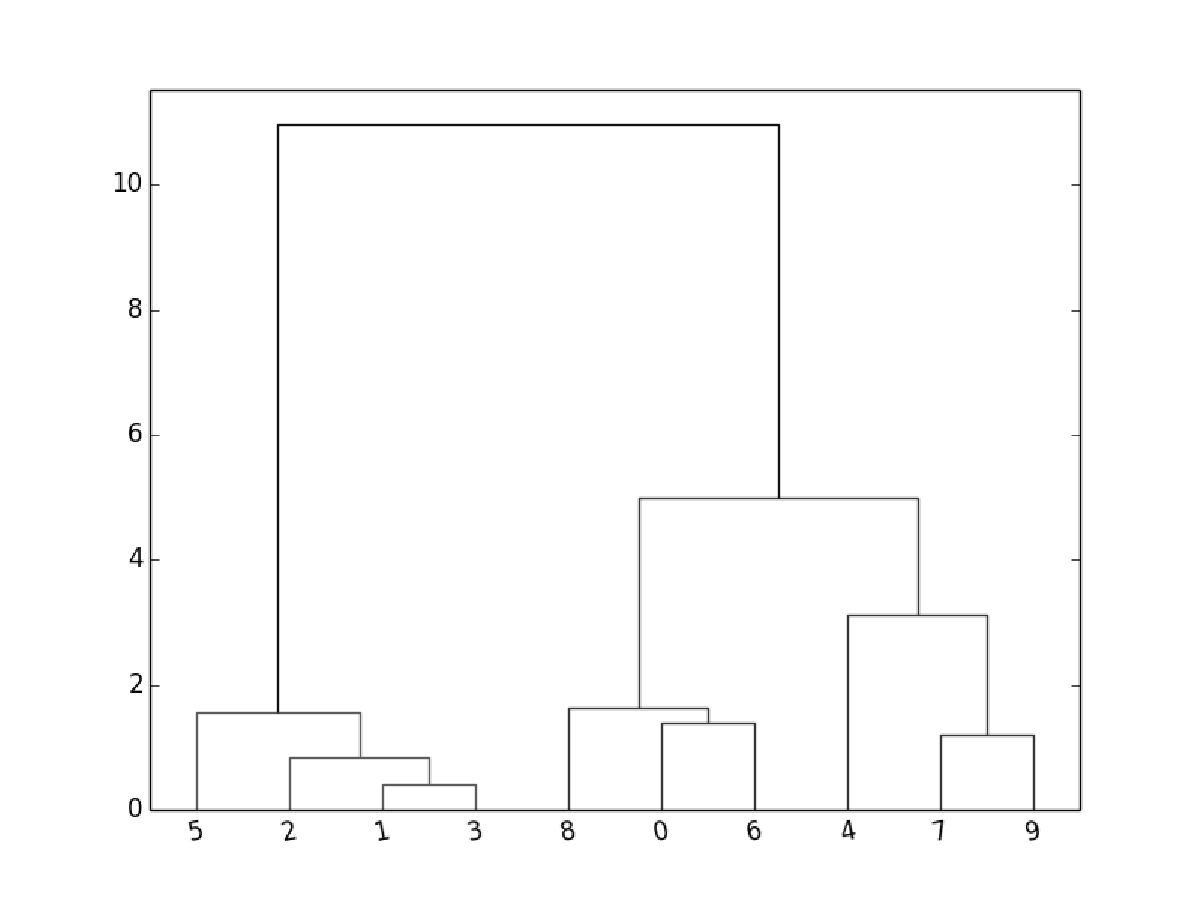
\includegraphics[width=0.8\textwidth]{images/pointer_representation.pdf}
    \caption{An example of the pointer representation of SLINK
        \cite{pointer-representation}. \label{fig:pointer-representation} }
\end{figure}

\newpage

\subsection{Algorithm}

The algorithm takes some data set $S$ with $n$ data points in it, and
utilizes three arrays of length $n$ to store the pointer representation.
These are called $\Pi. \Lambda, M$.

\begin{enumerate}
    \item Set $\Pi(n+1)$ to $n+1$, $\Lambda(n+1)$ to $\infty$.
    \item Set $M(i)$ to $d(i, n+1)$ for $i=1,...,n$.
    \item For $i$ increasing from $1$ to $n$ \\
        if $\Lambda(i) \geq M(i)$ \\
            set $M(\Pi(i))$ to $ min\{M(\Pi(i)), \Lambda(i)\}$ \\
            set $\Lambda(i)$ to $M(i)$ \\
            set $\Pi(i)$ to $n+1$ \\
        else \\
            set $M(\Pi(i))$ to $ min\{M(\Pi(i)), M(i)\}$ 
    \item For $i$ increasing from $1$ to $n$ \\\
        if $\Lambda(i) \geq \Lambda(\Pi(i))$ \\
            set $\Pi(1)$ to $n+1$.
\end{enumerate}

\begin{python}
def SLINK(S):
    points  = S.get_points()
    n       = len(points)
    
    pi, _lambda, M = [0]*n, [float("inf")]*n, [None]*n
    
    for i in range(1, n):
        pi[i] = i
        
        for j in range(i):
            M[j] = distance(points[i], points[j])
        
        for j in range(i):
            if _lambda[j] >= M[j]:
                M[pi[j]] = min(M[pi[j]], _lambda[pi[j]])
                _lambda[j] = M[j]
                pi[j] = i
            else:
                M[pi[j]] = min(M[pi[j]], M[j])
        
        for j in range(i):
            if _lambda[j] >= _lambda[pi[j]]:
                pi[j] = i
        
    return (_lambda, pi)
\end{python}

\newpage

\section{DBSCAN}

\emph{DBSCAN - Density Based Spatial Clustering of Applications with 
Noise} is an algorithm proposed by \citeauthor{DBSCAN} in 
\citeyear{DBSCAN}. It relies heavily on 6 definitions, which provides an 
outline for the algorithm.

Two input parameters are required, $\varepsilon$ which defines the 
neighborhood size of a point (see \ref{definition:eps-neigborhood}), and
$MinPts$ that determines the minimum number of points in a cluster.
These together define a notation of cluster density.

\subsection{Definitions}

\begin{definition}[$\varepsilon$-neighborhood of a point]
\label{definition:eps-neigborhood}
    The $\varepsilon$-neighborhood of a point $p$, denoted by
    $N_\varepsilon(p)$, is defined by 
    $$
        N_\varepsilon(p) = \{ q \in D | dist(p,q) \leq \varepsilon \}
    $$
\end{definition}

\begin{definition}[Directly Density-Reachable]
\label{definition:directly-density-reachable}
    A point $p$ is directly density-reachable from a point $q$ with 
    regard to $\varepsilon$ and $MinPts$ if
    \begin{enumerate}
      \item $ p \in N_\varepsilon(q) $ and
      \item $ |N_\varepsilon(q)| \geq MinPts $ (core point condition).
    \end{enumerate}
\end{definition}

\begin{definition}[Density-Reachable]
\label{definition:density-reachable}
    A point $p$ is density-reachable from a point $q$ with regard to
    $\varepsilon$ and $MinPts$ if there is a chain of points 
    $p_1, p_2, \ldots, p_n$, $p_1=q$, $p_n=p$ such that $p_{i+1}$ is
    directly density reachable from $p_i$.
\end{definition}

\begin{definition}[Density-Connected]
\label{definition:density-connected}
    A point $p$ is density-connected to a point $q$ with regard to
    $\varepsilon$ and $MinPts$ if there is a point $o$ such that both
    $p$ and $q$ are density-reachable from $o$ with regard to 
    $\varepsilon$ and $MinPts$.
\end{definition}

\begin{definition}[Cluster]
\label{definition:dbscan-cluster}
    Let $D$ be a database of points. A clustrer $C$ with regard to
    $\varepsilon$ and $MinPts$ is a non-empty subset of $D$ satisfying
    the following conditions:
    \begin{enumerate}
        \item $\forall p, q$: if $p \in C$ and $q$ is density-reachable
        from $p$ with regard to $\varepsilon$ and $MinPts$, then
        $q \in C$: Maximality)
        \item $\forall p, q \in C$: $p$ is density-connected to $q$ 
        with regard to $\varepsilon$ and $MinPts$.
    \end{enumerate}
\end{definition}

\begin{definition}[Noise]
\label{definition:dbscan-noise}
    Let $C_1,...C_k$ be the clusters of the database $D$ with regard
    to parameters $\varepsilon_i$ and $MinPts_i$, $i=1,...k$. Then we
    define the noise as the st of points in the database $D$ not 
    belonging to any cluster $C_i$, i.e. 
    $noise = \{ p \in D | \forall i: p \not\in C_i \}$ 
\end{definition}

\newpage

\subsection{Algorithm}
\begin{python}
def DBSCAN(S, eps, minPts)
	# The initial set of points S is initialized  
	# with clusterID set to UNCLASSIFIED.
	clusterID = nextId(NOISE)
	
	for point in S
		if point.clusterId == UNCLASSIFIED
			if expandCluster(S, point, clusterID, eps, minPts)
				clusterID = nextID(clusterID)

def expandCluster(S, point, clusterID, eps, minPts)
	seeds = S.regionQuery(point, eps)
	
	# Core point criterion not fulfilled for point, 
	# so this is temporary regarded as noise.
	if len(seeds) < minPts
		point.clusterID = NOISE
		return False
	
	for p in seeds
	    p.clusterID = clusterID
	
	seeds.remove(point)
	
	while not seeds.empty()
		current = seeds.pop()
		result = s.regionQuery(current, eps)
	
		if len(result) >= MinPts
			for p in result
				if p.clusterID in [UNCLASSIFIED, NOISE]
					if p.clusterID = UNCLASSIFIED
						seeds.append(p)
					p.clusterID = clusterID
	return True
\end{python}